%% $RCSfile: proj_proposal.tex,v $
%% $Revision: 1.3 $
%% $Date: 2016/06/10 03:44:08 $
%% $Author: kevin $

\documentclass[11pt, a4paper, twoside, openright]{report}

\usepackage{float} % lets you have non-floating floats
\usepackage{url} % for typesetting URLs
\usepackage{wrapfig}
\usepackage[image,ecs]{vuwproject}

\renewcommand{\thesection}{\arabic{section}}
\setlength{\parindent}{0pt}
\setlength{\parskip}{\baselineskip}

%  We don't want figures to float so we define
%
\newfloat{fig}{thp}{lof}[chapter]
\floatname{fig}{Figure}
\graphicspath{ {./Figures/} }

 

\title{Self Tuning Buck Converter}
\author{Niels Daniel Clayton}
\supervisor{Daniel Burmester}
\otherdegree{Honours of Electronic and Computer System Engineering}

\begin{document}

% Make the page numbering Roman, until after the contents, etc.
\frontmatter

%%%%%%%%%%%%%%%%%%%%%%%%%%%%%%%%%%%%%%%%%%%%%%%%%%%%%%%

\begin{abstract}

Switch-mode power supplies are commonly used in a wide variety of consumer and professional appliances to transform DC voltages with high efficiency. One such converter is the buck converter. The design of the buck converter requires specific components to design the output filter. These components be difficult to purchase or accurately manufacture. This project will implement a control system to actively control the switching frequency and eliminate the need design the output filter.   

\end{abstract}

%%%%%%%%%%%%%%%%%%%%%%%%%%%%%%%%%%%%%%%%%%%%%%%%%%%%%%%

\maketitle

\tableofcontents

% we want a list of the figures we defined
%\listof{fig}{Figures}

%%%%%%%%%%%%%%%%%%%%%%%%%%%%%%%%%%%%%%%%%%%%%%%%%%%%%%%

\mainmatter

%%%%%%%%%%%%%%%%%%%%%%%%%%%%%%%%%%%%%%%%%%%%%%%%%%%%%%%

\section{Introduction}


\subsection{Switch Mode Power Supplies}

Switch-mode power supplies convert a DC input voltage to another DC output voltage. They are commonly used in a wide variety of consumer and professional appliances such as laptops and chargers due to their high efficiency compared to other DC-to-DC converters. 

The step-down switch mode power supply also known as a buck converter, is a common DC-to-DC power converter that steps down an input voltage to the desired output efficiently. Currently, the design of these converters for specific applications requires a specifically designed output filter, designed around the switching speed of the converter. This filter will smooth the converter output voltage and maintain the inductor current ripple at the designed values. However this design process is not always applicable, if the specified components for the filter are not available there can be lead times, cost implications and delays.

\begin{figure}[h!]
  \begin{center}
    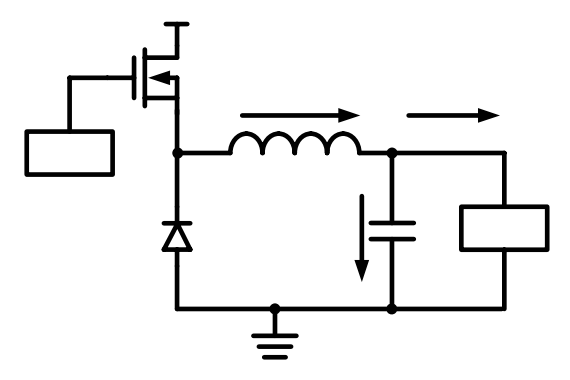
\includegraphics[width=0.6\linewidth]{asynchronous_buck.png} 
    \caption{Asynchronous buck converter topology \cite{BuckTopology}}
    \label{asynchronous_buck}
  \end{center}
\end{figure} 

This project aims to remove the need for designing the output stage of the buck converter. Using a control system, the switching frequency and duty cycle of the converter can be modulated to meet a selected inductor ripple, while maintaining a selected output voltage. This project will focus on the design and implementation of this control system on a basic asynchronous buck converter.  
\newpage

\section{The Problem}

The current buck converter design requires that a specific output filter be designed around the switching frequency of the converter, and the desired inductor ripple. This filter design process will often result in the designer requiring discrete passive components that are not easily available. This requirement for precise discrete components can greatly increase the cost of the converter, and can also cause delays in manufacturing due to the lead time of components.

Another side effect of this design process is that this desired inductor ripple will only be achieved at the designed output voltage or load. This means that in current buck converter designs, varying the output voltage, or output load will cause the inductor ripple to vary. This can lead to the buck converter no-longer meeting the required specifications, making it hard to design a converter for a complex load.

This project aims to eliminate the need to design the output stage of a buck converter. This will be achieved by implementing a control system to vary both the switching frequency and duty cycle, to achieve the desired inductor ripple and output voltage. This will allow the buck converter to actively adjust the switching frequency to match the currently designed output filter at all times.

\section{Proposed Solution}

The proposed solution to this problem will have 3 phases, the initial research and setup, the design, and the implementation phase. Each phase will have a selection of tasks that must be completed to be able to progress to the following phase. The following subsections will go into detail on the undertakings of each phase. For time estimations of each task please look at the Gantt chart in Figure \ref{fig:gantt}.

\subsection{Research and Setup}

The first phase of this project is the research and setup. The major component of this phase is the creation of the literature review that will be the basis of this project. In this literature review, I will compare and contrast a wide range of methods available to produce a frequency variable PWM signal. This review will also be used to compare and contrast varying sensing methods for sampling the inductor ripple and the output voltage. 

When the literature review is complete, I will select the methods of PWM generation and output sensing that are most suitable for this project. This will help me identify a range of components that I believe will be feasible for the design. These components will be purchased for used in the design phase. 

Finally, once the components have been purchased I will design a selection of development PCB's that will allow for simplistic interfacing with the purchased components and the existing buck converter design. This will help expedite the design phase.

\subsection{Design}
\label{sec:design}

In the design phase of the project, I will test and evaluate all of the selected PWM generation methods, and sensing methods. This will involve a large amount of prototyping on breadboards, along with possibly embedded programming on microcontrollers, and FPGA (Field Programmable Gate Array) design. The method of evaluation of these designs will be decided upon in the literature review.  

Once the evaluation of the designs is complete, I will make the final hardware selection. The components selected at this stage will be used to implement the closed-loop controller for the converter.

\subsection{Implementation}

Finally, in the implementation phase of the project, the finalised hardware design will be used to implement the closed-loop control system. This system will sample the inductor ripple and vary the switching speed and duty cycle of the buck converter to reach a requested ripple value. A Simulink simulation may be designed to help with the implementation and design of this controller.  

As the controller is being implemented, I will also design a final PCB for the buck converter. This PCB will include the entire buck converter design, with female headers for easy filter inductor and capacitor swapping.

\begin{figure}[!h]
  \begin{center}
    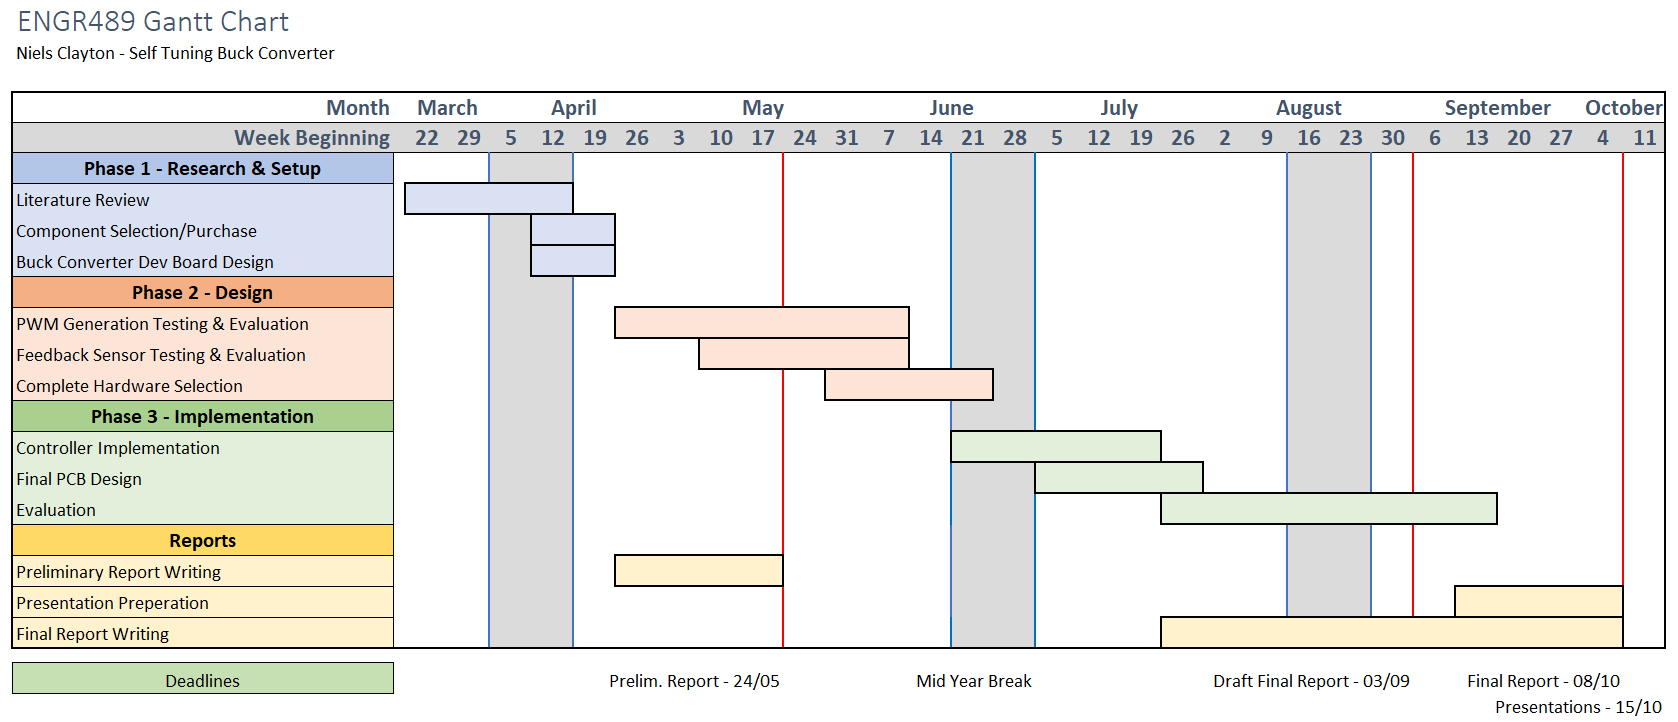
\includegraphics[width = \linewidth]{gantt.png} 
    \caption{Project Gantt Chart}
    \label{fig:gantt}
  \end{center}
\end{figure} 

\newpage
\section{Project Evaluation}

The evaluation of this project will be based upon meeting a pre-defined selection of specifications:

\begin{itemize}
  \item The buck converter will be capable of outputting up to 1A of current
  \item The buck converter will be able to take input voltages up to 12V DC
  \item The buck converter will be able to output between 3V and 10V DC
  \item The buck converter will have a switching frequency range from 1$kHz$ to 100$kHz$
  \item The user will be able to define the an output ripple between 5\% and 50\%, with increments of 1\%
\end{itemize}

\section{Safety and Resourcing}

\subsection{Safety Considerations}

Below in Table \ref{tab:hazzard} there is a safety hazard identification, prevention, and mitigation table.

\begin{table}[!h]
  \begin{tabular}{|l|l|l|}
  \hline
  \multicolumn{1}{|c|}{Potential Hazards}                                                         & \multicolumn{1}{c|}{Hazard Prevention}                                                                                                                                                                & \multicolumn{1}{c|}{Hazzard Mitigation}                                                                    \\ \hline
  \begin{tabular}[c]{@{}l@{}}Burns due to resistive\\ elements heating \\ during use.\end{tabular} & \begin{tabular}[c]{@{}l@{}}Ensure that no more than 5W of \\ power is dissipated across the \\ load at any time.\end{tabular}                                                                        & \begin{tabular}[c]{@{}l@{}}Turn off equipment that is \\ overheating.\end{tabular}                         \\ \hline
  \begin{tabular}[c]{@{}l@{}}Cuts due to misuse \\ of wire cutters\end{tabular}                    & \begin{tabular}[c]{@{}l@{}}Ensure that there are no \\ distractions when operating \\ potentially hazardous equipment.\end{tabular}                                                                  & \begin{tabular}[c]{@{}l@{}}Bandage the cut, and fill out \\ an accident/incident report.\end{tabular}      \\ \hline
  \begin{tabular}[c]{@{}l@{}}Burns due to misuse \\ of soldering iron\end{tabular}                 & \begin{tabular}[c]{@{}l@{}}Ensure that there are no \\ distractions when operating \\ potentially hazardous equipment. \\ Make sure to correctly store \\ the soldering iron after use.\end{tabular} & \begin{tabular}[c]{@{}l@{}}Apply ice to the burn and fill out \\ an accident/incident report.\end{tabular} \\ \hline
  Dangerous voltages                                                                               & \begin{tabular}[c]{@{}l@{}}Ensure that the power supply \\ never outputs more than the \\ maximum of 50V.\end{tabular}                                                                                & Turn off that is not operating safely                                                                     \\ \hline
  \end{tabular}
  \caption{Hazzard assessment }
  \label{tab:hazzard}
  \end{table}

\newpage
\subsection{Required Equipment}
\label{sec:equipment}
The Following list of equipment is currently available without purchase, but will be required for this project: 

\begin{itemize}
  \item Lab bench power supply
  \item Lab bench oscilloscope 
  \item Lab bench signal generator
  \item lab bench multi-meter
  \item Prototyping breadboards  
  \item Passive components (resistors, inductors, capacitors, MOSFETs, etc)
\end{itemize}

\subsection{Budget}

Below in Table \ref{tab:budget} is the total estimated cost of the components I will need to purchase for this project.

\begin{table}[!h]
  \begin{tabular}{|l|l|l|}
  \hline
  \multicolumn{1}{|c|}{Component} & \multicolumn{1}{c|}{Description}                                                           & Cost  \\ \hline
  PCB Manufacturing               & In house or external PCB manufacturing                                                     & \$50  \\ \hline
  Assorted components             & Parts to be tested and evaluated as discussed in section \ref{sec:design} & \$200 \\ \hline
  \end{tabular}
  \caption{Budget }
  \label{tab:budget}
  \end{table}

\subsection{Covid-19 Considerations}

Due to the effects of Covid-19 lockdowns, it is important to be prepared for the possible implication of going to the varying alert levels will have. 

In the case of alert level 2, the university will still be open and operating with enforced social distancing and masks. This alert level will have little to no effect on the progress of this project, as the honours lab allows for social distancing.

In the case of alert level 3 \& 4, the university will close. This means that I will not be able to access the honours lab to get to my equipment. In the case of alert level 3 or 4, I will have to ask the technicians if I am able to bring home with me the equipment listed in section \ref{sec:equipment} to continue working from home. If this is not possible then I will work to make an accurate simulation of the Project within Simulink. 


%%%%%%%%%%%%%%%%%%%%%%%%%%%%%%%%%%%%%%%%%%%%%%%%%%%%%%%
\backmatter
%%%%%%%%%%%%%%%%%%%%%%%%%%%%%%%%%%%%%%%%%%%%%%%%%%%%%%%

\bibliographystyle{ieeetr}
\bibliography{bibliography}
\end{document}
